\providecommand{\main}{..}
\documentclass[\main/main.tex]{subfiles}
\begin{document}

\chapter{Albero delle decisioni}
Si tratta di uno strumento di risoluzione per i problemi decisionali di tipo finito, che introduce una gerarchia sulle variabili di decisione e sulle variabili esogene.

Usando il \textbf{criterio del caso pessimo, Laplace o del valore atteso} si costruisce ponendo prima gli scenari e quindi le scelte (figura \ref{criterion_tree}).

\begin{figure}
  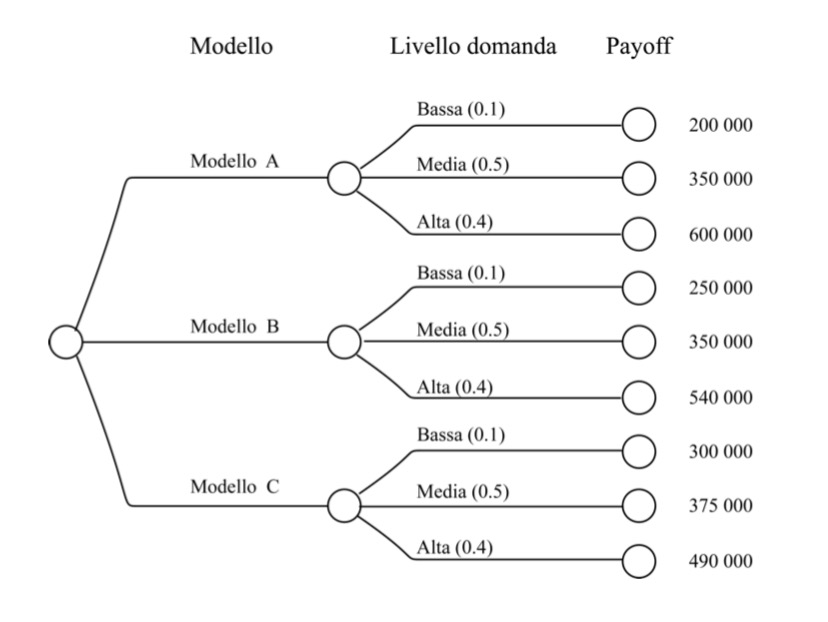
\includegraphics[width=0.5\textwidth]{criterion_tree}
  \caption{Albero delle decisioni}
  \label{criterion_tree}
\end{figure}

\end{document}